\chapter{Background}
\label{chap:background}

In this chapter we are going to explain the most important concepts of the 
upcoming 5G standard, talking about the Virtual Network Functions (VNFs) and 
how first experiments with this new technology already begun. Finally we are 
going to briefly introduce and explain the technologies involved and their role.

\section{Virtualization}
It is remarkable how cloud computing has surged in the recent years. This is due
the numerous features it carries, such as a great way to isolate processes and
mitigate possible attacks from malicious users. On top of that, it allows to run
``virtual'' machines with different configurations, without apporting any
changes to the host machine. Indeed, the virtualization concepts refer to the
property of a machine to be virtualized. To achieve this, the components that
forms a common computer need to be virtualized too. Thus, these assets are
recreated in this virtualized manner, e.g. Storage devices and computer network
resources~\cite{liu2014research}. At the time writing, there are two common
virtualization options: the virtualization through Hypervisor (defined also as
hypervisor-based) and the container virtualization.

\paragraph*{Hypervisor}
The first one is known for providing a very good isolation from the host
machine~\cite{eder2016hypervisor}, even if studies found possibilties for an
attacker to escape from the a virtual machine and operate on the host
machine\footnote{An example can be found in
  \url{https://github.com/MorteNoir1/virtualbox_e1000_0day}}. Even though every
component in a hypervisor environment is virtualized, there are possibilties for
the ``guest'' OS (the virtualized one), to access to physical devices (like USB
keys attacched on the ``host'' OS).

\paragraph*{Container-based}
Container-based virtualization uses a differnt approach to reach isolation.
Instead of creating a whole new stack, it applies very strict policies to the
programs running on the ``host'' machine. This concept has its roots back to the
jail environments, where group of process where isolated by the main OS, that
provided a virtualized filesystem~\cite{canonico2007virtualization}. In this
context, a container-based applications can be seen as a jailed application with
policies aimed to protect the host machine.

\begin{figure}[t]
  \centering
  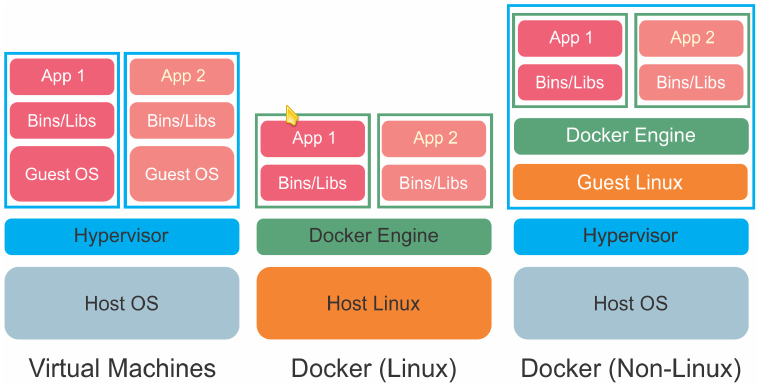
\includegraphics[scale=0.5]{docker_vs_hypervisor}
  \caption[Container-based emulation vs hypervisor emulation]{Container-based
    emulation, such as Docker vs hypervisor-based emulation~\cite{hung2016guidock}}
\end{figure}

\subsection{Network Virtulization}

Virtualization assumes another context when referred to networking: virtualized
networking allow multiple, heterogeneous networks to cohabit, increasing the
flexibility and manageability. This network separation creates two different
entities, that becomes decouples: who provides the infrastructure (commonly
called InPs) and who provides the services (SPs). A virtual network can be
create aggregating one or more InPs, thus creating a virtual network end-to-end
service~\cite{chowdhury2009network}. An example of this are the Virtual Private
Networks (VPNs), that are able to cross public networks, giving access to
content that otherwise would not be available locally.

\section{Software-defined networking}
The concept of Software-defined networking (SDN) is not new: starting from
1996~\cite{sezer2013we} it aims to provide user-controlled management of
forwarding in network nodes. This means to have the possibility to control the
forwarding procedures. A close examples of SDN implementations are Ethane and
OpenFlow, respectively created in 2007 and 2008. In an SDN architecture, there
is the decoupling of data and control plane\todo{ref}, but there is a
centralization of the networking logic and state~\cite{fundation2012software}.
The use of an SDN network is estimated to reduce the Capital Expenditure (CapEX)
and Operational Expenditure (OpEX) costs~\cite{benzekki2016software}.

\subsection{SDN stack}
\begin{figure}[ht]
 \centering
 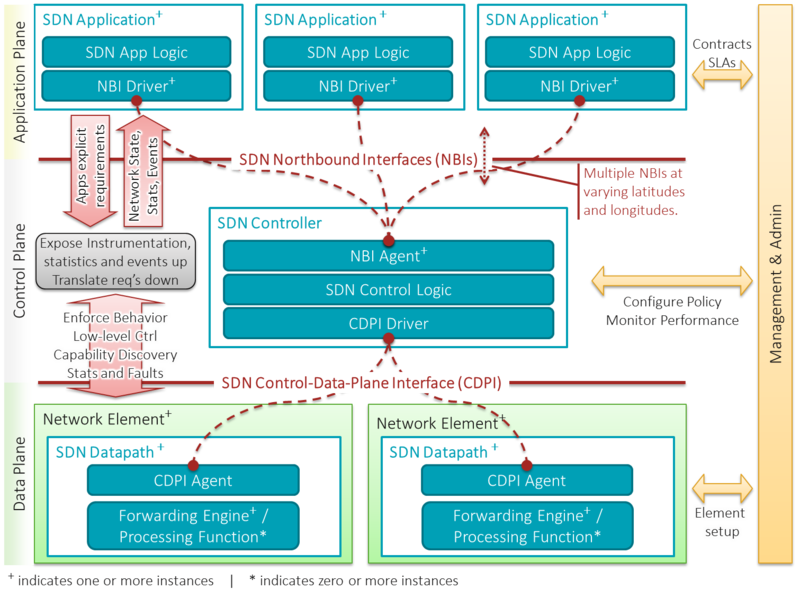
\includegraphics[scale=1.3]{sdn_architecture}
 \caption[SDN architecture schema]{SDN architecture schema. Is possible to 
denote the three layer logic: the Application plane, the Controller plane and 
the Data plane~\cite{fundation2013software}.}
 \label{chap:background:img:sdn_architecture}
\end{figure}

As the Figure~\ref{chap:background:img:sdn_architecture} illustrats, the SDN
architecture is formed by three layers, defined as planes, that accomplish
determinated tasks~\cite{fundation2012software} as
in~\cite{fundation2013software}. Below we will perform a brief exaplanation of
each plane.

\subsubsection{Application plane}
In general, this layer is responsible of abstracting the SDN network control
management~\cite{benzekki2016software}. The application plane holds SDN
applications, programs that have the possibility to change the way the SDN
network forwards the data. These applications have the possibility to access
hardware capabilities through specific API, that are called \emph{northbound}
interfaces (NBI). These interfaces usually, acts like a bridge between the SDN
applications and the SDN controllers and are usually implemented in an open and
vedor-neutral way~\cite{fundation2013software}.

\subsubsection{Control plane}
The SDN controllers, as just said in the previously, receives requests from the
SND applications. Since the controller is centralized, it can therefore exploit
the complete knowledge of the network. This gives the possibility to apply
networking optimizations like flow management~\cite{sezer2013we}. The controller
abstracts from the network complexity, and it can collect informations about the
network performing requests to the \emph{southbound} interfaces. The control
plane can have multiple controllers, that are in turn federated thanks to the
\emph{eastbound} and \emph{westbound} (e.g.
HyperFlow)~\cite{benzekki2016software}, that allow several existing controller
written with different languages to coexists.

\subsubsection{Data Plane}
The data plane is the lowest plane, and it provides the aforementioned
\emph{southbound} API. This kind of API can be deployed in two different kind of
scenarios: for in-band communications and for out-of-band
communications~\cite{benzekki2016software}. The data plane gives access to the
physical and virtual switches, routers and access-points, and it gives the
possibility to perform programmatic forwarding operations, but it is also able
to provide statistic reportings and it supports event notifications.

\subsection{OpenFlow protocol}
OpenFlow is an open communication protocols that enables the possibility to
actually program networks, offering the possibility to change the flow-tables
for layer 3 switches and for routers~\cite{mckeown2008openflow}. In other words,
the OpenFlow protocol gives the possibility for controller to access at these
components. Routes can be changed on the typology of the packet, or on the state
of the network (i.e. if a network is under heavy load, certain packages can be
discarded).

\begin{figure}[t]
 \centering
 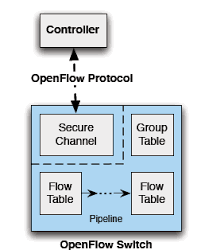
\includegraphics[scale=0.65]{openflow}
 \caption{OpenFlow protocol communication graph}
 \label{chap:background:img:openflow_protocol}
\end{figure}

In the Figure~\ref{chap:background:img:openflow_protocol} we have a
schematization of what we said before: every switch has a flow table that gets
updated thanks the OpenFlow protocol by the SDN controller, that is the one
managing the whole network.

\section{The upcoming connectivity standard: 5G}
The continuous innovation in the mobile network connectivity is leading to the
creation of a new standard, the 5G, which is estimated to arrive to the market
consumer in 2020~\cite{iwamura2015ngmn}. Lead by the Next Generation Mobile
Network (NGMN) alliance, a group composed by the major players in the field of
mobile connectivity, the 5G aims to offer not only at the end-user a new way to
browse the web, download and watch interactive content but also to create an
ad-hoc solution for Machine-to-Machine (M2M) data traffic, which is increasing
more than ever thanks to the spreading of IoT devices, which sensors need to
continuously send data to servers/data-centers. Relatively to \emph{Long Term
  Evolution} (LTE), 5G points to have data rates $10$ times better, with $10$
times smaller end-to-end latency and an increased connection density by $100$
times~\cite{alliance20155g}.

\begin{table}[t]
\centering
\resizebox{\textwidth}{!}{%
  \begin{tabular}{p{4,5cm}|p{5,5cm}|p{5cm}}
\textbf{Attribute}                                                    & 
\textbf{LTE capability}                                                         
 
                                                                           & 
\textbf{Improvement needed to meet NGMN requirements}                 \\ \hline
\textbf{Data rate (per user)}                                         & Up to 
100 Mb/s on average Peaks of 600 Mb/s (Cat 11/12).                              
 
                                                                     & 10X 
expected on average and peak rates and 100X expected on cell edge \\
\textbf{End-to-end latency}                                           & 10 ms 
for two-way RAN (pre-scheduled). Typically, up to 50 ms end-to-end if other 
factors are considered (e.g., transmission, CN, internet, proxy servers). & 10X 
(smaller)                                                         \\
\textbf{Mobility}                                                     & 
Functional up to 350 km/h (for certain bands up to 500 km/h). No support for 
civil aviation.                                                                
& 
1.5X                                                                  \\
\textbf{\begin{tabular}[c]{@{}l@{}}Connection\\ density\end{tabular}} & 
Typically $\sim$2,000 active users/km2.                                         
 
                                                                           & 
100X                                                                 
\end{tabular}%
}
\caption[5G improvement over LTE]{An extract from the official 5G white paper 
illustrating the improvements of 5G relatively to LTE connections.}
\label{chap:intro:table:ltevs5g}
\end{table}

Part of the new requirements can be satisfied using a large radio spectrum with
higher frequencies. The utilization of higher frequencies, though, mean that the
radio signals can be easily disrupted by physical objects, like buildings and
many geographical elements (such as hills and mountains), clashing with the
expectation of an ever-reachable connectivity. It is here where virtualization
plays an important role. In fact, the re-design of some network components today
existing via hardware can transform a monolithic networking approach to a 
modular one, exploiting the flexibility that Virtual Network Functions 
(VNFs)\cite{moens2014vnf} can offer thanks to virtualization, closing the gap to
the use-case fulfillment defined by the NGMN alliance~\cite{iwamura2015ngmn}
which require a decreased time to set up and deploy network services
(specifically, from 90 hours to 90 minutes~\cite{networld20202014role}).

\subsection{5G architecture}

With the constraints placed on the requirements formulated by the NGMN alliance,
5G envisage a multi-layered architecture, based on three main
layers~\cite{alliance20155g}:
\begin{itemize}
\item \textbf{infrastructure resource layer}: physical resources that are 
exposed via a virtualized interface, and that can be monitored using specific 
APIs
\item \textbf{business enablement layer}: where a library of functions and
  deployment is contained, and its configuration is accessible via APIs
\item \textbf{business application layer}: layer that contains specific
  applications and services of the operator
\end{itemize}

\begin{figure}[t]
  \centering
  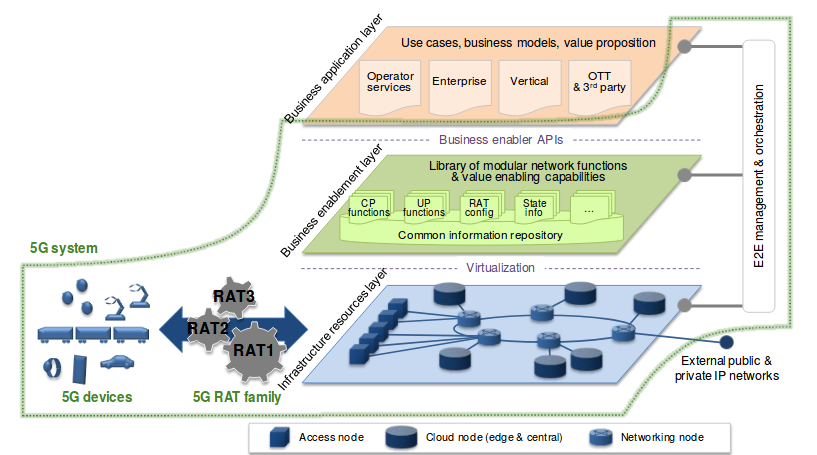
\includegraphics[scale=0.55]{5garchitecture}
  \caption[5G Architecture]{5G Architecture~\cite{alliance20155g}}
  \label{chap:background:img:5garchitecture}
\end{figure}

This separation in layers allows to easily manage multiple identities 
differently: an Internet Service Provider (ISP) could manage a multitude of 
physical infrastructures and have multiple business enablements dislocated 
along an entire continent for example, but it could decide to have only a 
single centralized business application deployment that manage all the other 
layers resources.

\subsubsection{Network slicing}
The role of a \emph{network slice} in a 5G architecture is to specifically
handle the Control-plane of a particular service (e.g. smartphones traffic,
autonomous driving, massive IoT), deploying resources in a manner that assure
the required latency, security and reliability. While some very peculiar and
legacy service could require specific hardware, the common resources between
services could be shared in a virtualized way, providing auto-scaling
capabilities in services that are under heavy network pressure.

\section{The VIBES project}
This thesis started as a part of the VIBES project~\cite{vibesesa}, whose main
requirement is to enhance the performance of end-to-end IP based that involves
satellite connections. To reach this goal, the project specifications suggest to
exploit the 5G incoming technology and use the NFV-MANO architecture to perform
first packets elaboration and performance improvement and finally TCP/IP
satellite chunk optimization with the Performance Enhancing Proxy (PEP). The
VIBES project proposed five technical requirements:
\begin{enumerate}
  \item Analysis of the applicability of current and new Internet protocols in
  the proposed VNF-PEP architecture
  \item Implementation of a VNF-PEP prototype
  \item Building of a PoC test platform
  \item VNF-PEP validation and performance tests on 5G use-cases
  \item Demonstration test-bed management
\end{enumerate}

\begin{figure}[t]
 \centering
 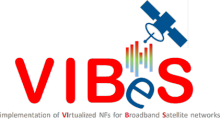
\includegraphics[scale=1]{vibes_logo}
 \caption{ViBeS project logo}
 \label{chap:background:img:vibes_logo}
\end{figure}

\subsection{VNF-PEP architecture and internet protocols}
VNF-PEP is the softwarization of the usual PEP technology. One of the goals of
the project is to research and include this technology in the usual VNF
ecosystem to include without change satellite communications to the SFC. The
architecture of the systems will be based on clusters of containers whose
management and orchestration will follows the ETSI MANO architecture and SDN
principles. Thanks to VNF-PEP will be possible to dynamically take decisions on
how to optimize a certain communication.

%The analysis of this topic revealed to be trivial: since internet has many
%different protocols that would become infeasible to support all of them at the
%same time, packet encapsulation present itself as the only feasible solution:
%every packet incoming in the VNFs has already been encapsulated by a generic
%packet encapsulator/decapsulator,
%\todo{Also I think that the main purpose of UDP encapsulation is not to hide 
%the protocol used on the edges but 1) use a ``quick protocol to exchange data 
%among VNFs and 2) we are hiding the path not the protocol itself. As we were 
%discussing, we are creating some sort of proxy, so the aim will be the same 
%even if we support a plethora of protocols.''} making the whole architecture 
%independent from the protocol a particular flux of data. To achieve this, 
%several solutions have been studied, and at the end packet encapsulation with 
%TCP split (for TCP sessions) have been chosen. The rationale that guided us on 
%this choice is described in Chapter~\ref{chap:vnf_ns_impl}. \todo{Update 
%reference with the section of the explanation}
%
%\subsection{VNF-PEP prototype}
%
%Since the requirement for the whole system (MANO+PEP) were too challenging, the 
%goal shifted into creating a MANO test-bed and a working NFVI, excluding PEP. 
%The VNF architecture was shaped following the container orchestrator we decided 
%to use. An more detailed architectural implementation can be found at 
%Chapter~\ref{chap:archimpl}.
%
%\vspace{0.5cm}
%
%Starting with the first step of creating a MANO able to process incoming data
%packets through VNF functions, we encountered that many networking tools already
%present in the market required some tweaking and some integration, shifting our
%goal to create a complete European Telecommunications Standards Institutes
%(ETSI) Management and orchestrator (MANO) test-bed instead, following the
%specifications suggested in the RFC 7665, thus implementing only the first three
%requisites, without digging in the satellite data flow optimization. In
%particular, we discovered how, these tools, were suitable to create ETSI MANO
%and VNFs using virtual machine or exploiting cloud technologies, while they were
%not designed with enough flexibility an integration with Docker. In the next
%chapter we are going to take a deep analysis of the cited technologies 
%(Section~\ref{chap:prjan:sec:tech}, in order to provide to the reader enough 
%context to be able to understand our design choices we are going to describe 
%later.
%
%\noindent With this in mind, we performed a requirements analysis described in
%the next chapter.\todo{This should be put at the end of the introduction.}
% 
